% !TEX program = lualatex
% !TEX options = -synctex=1 -interaction=nonstopmode -file-line-error -shell-escape -halt-on-error %DOC%
% !TEX encoding = UTF-8 Unicode

\documentclass[twoside, 12pt, a4paper]{extreport}
\usepackage{geometry}
\geometry{
	left=15mm,
	right=15mm,
	top=12mm,
	bottom=15mm,
	marginparwidth=0mm,
	marginparsep=0mm
	}
	
\newcommand{\wstawplik}[1]{\input{../../include/#1}}%skraca kod
\wstawplik{headerofficium-kopia}
% elementy zmienne co do headerofficium:
\graphicspath{{../../img/}} % katalog obrazów
%\svgpath{{../include/}}
\grechangestaffsize{20}%rozmiar wyniku GregorioTEX
\grechangestyle{initial}{\greIniZallmanCaps\fontsize{36}{20}\selectfont} % ustawia czcionkę zdefiniowaną w sekcji czcionek o zmniejsza wielkość
\gresetlastline{ragged}
% koniec 

% debugowanie:
% %\iffalse %*** %\fi %***
% \tracingall przed problematycznym kodem - bardzo dużo informacji
% lualatex+se+debug - dodatkowe opcje: -file-line-error i -halt-on-error 
% \errorcontextlines
\def\mydebug{1}% 0 - debugowanie, 1 - bez debugowania (wyłącza bloki \if\mydebug1)
\begin{document}
\pagestyle{plain}	
\fontspec{times}
\large
\titlespacing*{\chapter}{0pt}{0pt}{5pt}	
\titleformat{\chapter}[hang]{\filcenter\LARGE\scshape\bfseries}{}{0pt}{} % format nagłówków
\titlespacing*{\section}{0pt}{0pt}{0pt}	
\titleformat{\section}[hang]{\filcenter\large\scshape}{}{0pt}{} % format nagłówków

\setlength{\parindent}{0pt}
\gresetbracerendering{font}

\pagenumbering{gobble} % nie jest wyprowadzany żaden numer strony, chociaż numer jest nadal resetowany. Odniesienia do tej strony również są puste.

%% ----------------- STRONA TYTUŁOWA  ---------------------
\begin{center}
	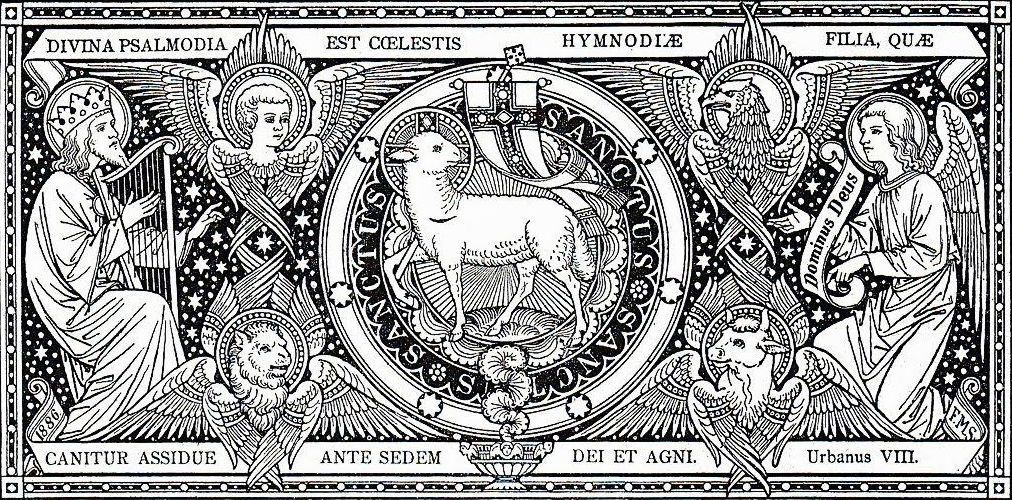
\includegraphics[width=1.0\textwidth]{divina_psalmodia.jpg}
	\vfill
	\fontspec{jsl-ancient.ttf}
	\fontsize{20}{40}\selectfont
	{Ad I VESPERAS}\par
	\fontsize{46}{50}\selectfont
	{In Conceptione Immaculata Beatæ Mariæ Virginis}\par
	\fontsize{20}{40}\selectfont
	{Commemoratio: Dominica II Adventus}\par
	\vfill
	\large\textit{Liber usualis, Solesmes, 1961, p.1320}
\end{center}
\pagebreak
\thispagestyle{empty}
\sekcja{Ante Divinum officium}{Odmawia się po cichu w pozycji klęczącej kreśląc znak krzyża na ustach.}%
\BeginParallel{0.5}
	\latN{\inicjal{A}{péri},~\red{\grecross}~Dómine, méum ad benedicéndum nómen sánctum túum: múnda quoqúe cor méum ab ómnibus vánis, pervérsis et aliénis cogitatiónibus; intelléctum illúmina, afféctum inflámma, ut dígne, atténte ac devóte hoc Offícium recitáre váleam, et exaudíri mérear ánte conspéctum divínae Majestátis túae. Per Chrístum Dóminum nóstrum. Amen.\linespace}
	\polN{\inicjal{O}{twórz},~\red{\grecross}~Panie, usta moje, dla błogosławienia świętego imienia Twego: oczyść także serce moje od wszelkich myśli próżnych, przewrotnych i~niewłaściwych; oświeć rozum, rozpal uczucie, abym godnie, uważnie i~pobożnie mógł odmówić to oficjum, i~zasłużył na wysłuchanie przed obliczem Twego Boskiego majestatu. Przez Chrystusa, Pana naszego. Amen.\linespace}
 	\latN{\inicjal{D}{ómine}, in unióne illíus divínae intentiónis, qúa ípse in térris laúdes Déo persolvísti, hanc tíbi Hóram persólvo.}
	\polN{\inicjal{P}{anie}, w~zjednoczeniu z~tą Boską intencją, z~którą Ty sam, na ziemi będąc, chwałę Bogu zanosiłeś, Tobie te godziny zanoszę.}
\EndParallel
\dekor{0.4}{amdg800x533.jpg}
\pagebreak
%% -----------------  INCIPIT ---------------------
\large
\setstretch{1.1} 
\begin{spacing}{0.7}
\begin{center}
	\fontspec{Libertinus Serif}
	\section*{Incipit}
%	\red{\small\textit{ewentualne rubryki}}
	\vspace{10mm}
\end{center}	
\end{spacing}
\gresetinitiallines{0}
\gabcsnippet{(c4) <c><sp>V/</sp>.</c> De(f)us(g_[uh:l]h) (,) <c><v>\grecross</v></c>  in(h) ad(h)ju(h)tó(h)ri(h)um(h) me(ixg!hwi)um(h) in(h)tén(hg)de.(gh..) (::)}
\gabcsnippet{(c4) <c><sp>R/</sp>.</c> Dó(f)mi(gh)ne(h'_) (,) ad(h) ad(h)ju(h)ván(h)dum(h) me(ixg!hwi) fe(h)stí(hg)na.(gh..) (::)}
\gabcsnippet{(c4)Gló(f)ri(gh)a(h) Pa(h)tri,(h) et(h) Fí(h)li(h)o,(h'_) (,) et(h) Spi(h)rí(ixg!hwi)tu(h)i(h) San(hg)cto.(gh..) (:) 
Sic(f)ut(gh) e(h)rat(h) in(h) prin(h)cí(h)pi(h)o,(h'_) (,) et(h) nunc,(ixg!hwi) et(h) sem(hg)per,(gh..) (;) et(h) in(h) saé(h)cu(h)la(h) sae(h)cu(h)ló(h)rum.(ixi) A(h)men.(g.) (;) 
Al(h)le(ixi)lú(hg~){ia}.(g.) (::)}
\vspace{10mm}

%% -----------------  PSALMI ---------------------
\begin{spacing}{0.7}
\begin{center}
	\fontspec{Libertinus Serif}
	\section*{Psalmi}
%	\red{\small\textit{ewentualne rubryki}}
	\vspace{10mm}
\end{center}	
\end{spacing}
%% --- 1. Psalm 109 - 1 g2------
\red{\large{Psalm 109}\vspace{4mm}}
\gresetinitiallines{1}\greannotation{1. Ant.}\greannotation{1. g2}\gabcsnippet{(c4) TO(f')TA(f) pul(h)chra(h) es(ixi') Ma(g)rí(g)a,(f_h) <c><v>\greheightstar</v></c>(;) et(hf~) má(g)cu(f)la(d) o(f)ri(e')gi(f)ná(gh)lis(ghg___) (,) non(fe) est(fg) in(ef~) te.(d.) (::)}
\vspace{4mm}
\greannotation{Psalm}\greannotation{109}\gabcsnippet{(c4) Di(f)xit(gh) Dó(h)mi(h)nus(h) <b>Dó</b>(ixi)mi(hr)no(h) <b>me</b>(g hr)o:(h.) <c><v>\greheightstar</v></c>(:) Se(h)de(h) a(h) <i>dex</i>(g)<i>tris</i>(f) <b>me</b>(g gr)is:(ghg.) (::)}
\begin{enumerate}[start=2]
\begin{spacing}{0.8}
\item Donec ponam ini\textbf{mí}cos \textbf{tu}os,~\red{*} scabéllum pe\textit{dum} \textit{tu}\textbf{ó}rum.
\item Virgam virtútis tuæ emíttet Dómi\textbf{nus} ex \textbf{Si}on:~\red{*} domináre in médio inimicó\textit{rum} \textit{tu}\textbf{ó}rum.
\item Tecum princípium in die virtútis tuæ in splendóri\textbf{bus} sanc\textbf{tó}rum:~\red{*}  ex útero ante lucíferum \textit{gé}\textit{nu}\textbf{i} te.
\item Jurávit Dóminus, et non pœni\textbf{té}bit \textbf{e}um:~\red{*} Tu es sacérdos in ætérnum secúndum órdi\textit{nem} \textit{Mel}\textbf{chí}sedech.
\item Dóminus a \textbf{dex}tris \textbf{tu}is,~\red{*}  confrégit in die iræ \textit{su}\textit{æ} \textbf{re}ges.
\item Judicábit in natiónibus, im\textbf{plé}bit ru\textbf{í}nas:~\red{*} conquassábit cápita in ter\textit{ra} \textit{mul}\textbf{tó}rum.
\item De torrénte in \textbf{vi}a \textbf{bi}bet:~\red{*} proptérea exal\textit{tá}\textit{bit} \textbf{ca}put.
\item Glória \textbf{Pa}tri, et \textbf{Fí}lio,~\red{*} et Spirí\textit{tu}\textit{i} \textbf{Sanc}to.
\item Sicut erat in princípio, et \textbf{nunc}, et \textbf{sem}per,~\red{*} et in sǽcula sæcu\textit{ló}\textit{rum}. \textbf{A}men.
\end{spacing}
\end{enumerate}
\gresetinitiallines{1}\greannotation{1. Ant.}\greannotation{1. g2}\gabcsnippet{(c4) TO(f')TA(f) pul(h)chra(h) es(ixi') Ma(g)rí(g)a,(f_h) (;) et(hf~) má(g)cu(f)la(d) o(f)ri(e')gi(f)ná(gh)lis(ghg___) (,) non(fe) est(fg) in(ef~) te.(d.) (::)}
\vspace{6mm}

%% --- 2. Psalm 112 - 8G ---
\red{\large{Psalm 112}\vspace{4mm}}
\gresetinitiallines{1}\greannotation{2. Ant.}\greannotation{8. G}\gabcsnippet{(c4) VE(g)sti(f)mén(hj)tum(i') tu(g)um(g'_) <c><v>\greheightstar</v></c>(,) cán(h)di(g)dum(fh) qua(j)si(j) nix,(ij..) (;) et(hg~) fá(h)ci(g)es(e_f) tu(g)a(gf) sic(gh)ut(h) sol.(g.) (::)}
\vspace{4mm}
\greannotation{Psalm}\greannotation{112}\gabcsnippet{(c4) Lau(g)dá(h)te,(j) pú(j)e(j)ri,(j) <b>Dó</b>(k)mi(jr)num:(j.) <c><v>\greheightstar</v></c>(:) lau(j)dá(j)te(j) <i>no</i>(i)<i>men</i>(j) <b>Dó</b>(h)mi(gr)ni.(g.) (::)}
\begin{enumerate}[start=2]
\begin{spacing}{0.8}
\item Sit nomen Dómini bene\textbf{díc}tum,~\red{*} ex hoc nunc, et us\textit{que} \textit{in} \textbf{sǽ}culum.
\item A solis ortu usque ad oc\textbf{cá}sum,~\red{*} laudábile \textit{no}\textit{men} \textbf{Dó}mini.
\item Excélsus super omnes gentes \textbf{Dó}minus,~\red{*} et super cælos gló\textit{ri}\textit{a} \textbf{e}jus.
\item Quis sicut Dóminus, Deus noster, qui in altis \textbf{há}bitat,~\red{*} et humília réspicit in cælo \textit{et} \textit{in} \textbf{ter}ra?
\item Súscitans a terra \textbf{ín}opem,~\red{*} et de stércore é\textit{ri}\textit{gens} \textbf{páu}perem:
\item Ut cóllocet eum cum prin\textbf{cí}pibus,~\red{*} cum princípibus pó\textit{pu}\textit{li} \textbf{su}i.
\item Qui habitáre facit stérilem in \textbf{do}mo,~\red{*} matrem filió\textit{rum} \textit{læ}\textbf{tán}tem.
\item Glória Patri, et \textbf{Fí}lio,~\red{*} et Spirí\textit{tu}\textit{i} \textbf{Sanc}to.
\item Sicut erat in princípio, et nunc, et \textbf{sem}per,~\red{*} et in sǽcula sæcu\textit{ló}\textit{rum}. \textbf{A}men.
\end{spacing}
\end{enumerate}
\gresetinitiallines{1}\greannotation{2. Ant.}\greannotation{8. G}\gabcsnippet{(c4) VE(g)sti(f)mén(hj)tum(i') tu(g)um(g'_) (,) cán(h)di(g)dum(fh) qua(j)si(j) nix,(ij..) (;) et(hg~) fá(h)ci(g)es(e_f) tu(g)a(gf) sic(gh)ut(h) sol.(g.) (::)}
\vspace{6mm}

%% --- 3. Psalm 121 - 8c ---
\red{\large{Psalm 121}\vspace{4mm}}
\gresetinitiallines{1}\greannotation{3. Ant.}\greannotation{8. c}\gabcsnippet{(c3) TU(h) gló(gh)ri(f)a(f) Je(ed)rú(ef)sa(f)lem,(e.) <c><v>\greheightstar</v></c>(,) tu(e) lae(e)tí(f')ti(e)a(d') Is(e)ra(e)el,(f.) (;) tu(f) ho(d')no(f)ri(h)fi(g)cén(h_i)ti(h)a(hg/hih.) (,) pó(f_h)pu(h)li(g) no(e.)stri.(e.) (::)}
\vspace{4mm}
\greannotation{Psalm}\greannotation{121}\gabcsnippet{(c3) Læ(e)tá(f)tus(h) sum(h) in(h) his,(h) quæ(h) dic(h)ta(h) sunt(h) <b>mi</b>(i hr)hi:(h.) <c><v>\greheightstar</v></c>(:) In(h) do(h)mum(h) Dó(h)<i>mi</i>(f)<i>ni</i>(h) <b>í</b>(i)bi(hr)mus.(h.) (::)}
\begin{enumerate}[start=2]
\begin{spacing}{0.8}
\item Stantes erant pedes \textbf{nos}tri,~\red{*} in átriis tu\textit{is}, \textit{Je}\textbf{rú}salem.
\item Jerúsalem, quæ ædificátur ut \textbf{cí}vitas:~\red{*} cujus participátio ejus \textit{in} \textit{id}\textbf{íp}sum.
\item Illuc enim ascendérunt tribus, tribus \textbf{Dó}mini:~\red{*} testimónium Israël ad confiténdum nó\textit{mi}\textit{ni} \textbf{Dó}mini.
\item Quia illic sedérunt sedes in ju\textbf{dí}cio,~\red{*} sedes super \textit{do}\textit{mum} \textbf{Da}vid.
\item  Rogáte quæ ad pacem sunt Je\textbf{rú}salem:~\red{*} et abundántia dili\textit{gén}\textit{ti}\textbf{bus} te:
\item Fiat pax in virtúte \textbf{tu}a:~\red{*} et abundántia in túr\textit{ri}\textit{bus} \textbf{tu}is.
\item Propter fratres meos, et próximos \textbf{me}os,~\red{*} loquébar \textit{pa}\textit{cem} \textbf{de} te:
\item Propter domum Dómini, Dei \textbf{nos}tri,~\red{*} quæsívi \textit{bo}\textit{na} \textbf{ti}bi.
\item Glória Patri, et \textbf{Fí}lio,~\red{*} et Spirí\textit{tu}\textit{i} \textbf{Sanc}to.
\item Sicut erat in princípio, et nunc, et \textbf{sem}per,~\red{*} et in sǽcula sæcu\textit{ló}\textit{rum}. \textbf{A}men.
\end{spacing}
\end{enumerate}
\gresetinitiallines{1}\greannotation{3. Ant.}\greannotation{8. c}\gabcsnippet{(c3) TU(h) gló(gh)ri(f)a(f) Je(ed)rú(ef)sa(f)lem,(e.) (,) tu(e) lae(e)tí(f')ti(e)a(d') Is(e)ra(e)el,(f.) (;) tu(f) ho(d')no(f)ri(h)fi(g)cén(h_i)ti(h)a(hg/hih.) (,) pó(f_h)pu(h)li(g) no(e.)stri.(e.) (::)}
\vspace{6mm}

%% --- 4. Psalm 126 - 7a ---
\red{\large{Psalm 126}\vspace{4mm}}
\gresetinitiallines{1}\greannotation{4. Ant.}\greannotation{7. a}\gabcsnippet{(c3) BE(e)ne(e)dí(hg)cta(h) es(i_[uh:l]j) tu,(i'_[oh:h]) <c><v>\greheightstar</v></c>(,) Vir(h)go(j') Ma(k)rí(ji)a,(i.) (;) a(hg) Dó(fi)mi(i)no(i') De(j)o(h) ex(hg)cél(e)so(e_[uh:l]f) (;) prae(df) ó(h)mni(g')bus(h) mu(i')li(h)é(ij)ri(i)bus(hv_GF) su(g)per(f) ter(e.)ram.(e.) (::)}
\vspace{4mm}
\greannotation{Psalm}\greannotation{126}\gabcsnippet{(c3) Ni(hg)si(hi) Dó(i)mi(i)nus(i) æ(i)di(i)fi(i)<b>cá</b>(k)ve(jr)rit(j) <b>do</b>(i jr)mum,(j.) <c><v>\greheightstar</v></c>(:) in(i) va(i)num(i) la(i)bo(i)ra(i)vé(i)runt(i) qui(i) æ(i)<b>dí</b>(j)fi(ir)cant(i) <b>e</b>(h hr)am.(gf..) (::)}
\begin{enumerate}[start=2]
\begin{spacing}{0.8}
\item Nisi Dóminus custodíerit \textbf{ci}vi\textbf{tá}tem,~\red{*} frustra vígilat qui cus\textbf{tó}dit \textbf{e}am.
\item Vanum est vobis ante \textbf{lu}cem \textbf{súr}gere:~\red{*} súrgite postquam sedéritis, qui manducátis \textbf{pa}nem do\textbf{ló}ris.
\item Cum déderit diléctis \textbf{su}is \textbf{som}num:~\red{*} ecce heréditas Dómini fílii: merces, \textbf{fruc}tus \textbf{ven}tris.
\item Sicut sagíttæ in \textbf{ma}nu pot\textbf{én}tis:~\red{*} ita fílii \textbf{ex}cus\textbf{só}rum.
\item Beátus vir qui implévit desidérium \textbf{su}um ex \textbf{ip}sis:~\red{*} non confundétur cum loquétur inimícis \textbf{su}is in \textbf{por}ta.
\item Glória \textbf{Pa}tri, et \textbf{Fí}lio,~\red{*} et Spi\textbf{rí}tui \textbf{Sanc}to.
\item Sicut erat in princípio, et \textbf{nunc}, et \textbf{sem}per,~\red{*} et in sǽcula sæcu\textbf{ló}rum. \textbf{A}men.
\end{spacing}
\end{enumerate}
\gresetinitiallines{1}\greannotation{4. Ant.}\greannotation{7. a}\gabcsnippet{(c3) BE(e)ne(e)dí(hg)cta(h) es(i_[uh:l]j) tu,(i'_[oh:h]) (,) Vir(h)go(j') Ma(k)rí(ji)a,(i.) (;) a(hg) Dó(fi)mi(i)no(i') De(j)o(h) ex(hg)cél(e)so(e_[uh:l]f) (;) prae(df) ó(h)mni(g')bus(h) mu(i')li(h)é(ij)ri(i)bus(hv_GF) su(g)per(f) ter(e.)ram.(e.) (::)}
\vspace{6mm}

%% --- 5. Psalm 147 - 3a2 ---
\red{\large{Psalm 147}\vspace{4mm}}
\gresetinitiallines{1}\greannotation{5. Ant.}\greannotation{3. a2}\gabcsnippet{(c4) TRa(e_[oh:h][ll:1]d)he(g) nos(h_j) <c><v>\greheightstar</v></c>(,) Vir(i')go(j) im(k)ma(j')cu(i)lá(hi)ta,(hg..) (;) post(g) te(hj) cur(i)ré(g!hwi_[oh:h]g)mus(h'_) (,) in(g) o(e)dó(fg)rem(g) un(g)guen(h)tó(gf)rum(g) tu(gf)ó(e.)rum.(e.) (::)}
\vspace{4mm}
\greannotation{Psalm}\greannotation{147}\gabcsnippet{(c4) Lau(g)da,(hj) Je(j)<b>rú</b>(k)sa(jr)lem,(j) <b>Dó</b>(jr[ocb:1{])<b>mi</b>(ih[ocb:0}])num:(j.) <c><v>\greheightstar</v></c>(:) lau(j)da(j) De(j)um(j) <i>tu</i>(ji)<i>um</i>,(hi) <b>Si</b>(h gr)on.(gh..) (::)}
\begin{enumerate}[start=2]
\begin{spacing}{0.8}
\item Quóniam confortávit seras por\textbf{tá}rum tu\textbf{á}rum:~\red{*} benedíxit fíliis \textit{tu}\textit{is} \textbf{in} te.
\item Qui pósuit fines \textbf{tu}os \textbf{pa}cem:~\red{*} et ádipe fruménti \textit{sá}\textit{ti}\textbf{at} te.
\item Qui emíttit elóquium \textbf{su}um \textbf{ter}ræ:~\red{*} velóciter currit \textit{ser}\textit{mo} \textbf{e}jus.
\item Qui dat nivem \textbf{sic}ut \textbf{la}nam:~\red{*} nébulam sicut cí\textit{ne}\textit{rem} \textbf{spar}git.
\item Mittit crystállum suam \textbf{sic}ut buc\textbf{cél}las:~\red{*} ante fáciem frígoris ejus quis \textit{sus}\textit{ti}\textbf{né}bit?
\item Emíttet verbum suum, et lique\textbf{fá}ciet \textbf{e}a:~\red{*} flabit spíritus ejus, et \textit{flu}\textit{ent} \textbf{a}quæ.
\item Qui annúntiat verbum \textbf{su}um \textbf{Ja}cob:~\red{*} justítias, et judícia \textit{su}\textit{a} \textbf{Is}raël.
\item Non fecit táliter omni \textbf{na}ti\textbf{ó}ni:~\red{*} et judícia sua non manifes\textit{tá}\textit{vit} \textbf{e}is.
\item Glória \textbf{Pa}tri, et \textbf{Fí}\textbf{li}o,~\red{*} et Spirí\textit{tu}\textit{i} \textbf{Sanc}to.
\item Sicut erat in princípio, et \textbf{nunc}, et \textbf{sem}per,~\red{*} et in sǽcula sæcu\textit{ló}\textit{rum}. \textbf{A}men.
\end{spacing}
\end{enumerate}
\gresetinitiallines{1}\greannotation{5. Ant.}\greannotation{3. a2}\gabcsnippet{(c4) TRa(e_[oh:h][ll:1]d)he(g) nos(h_j) (,) Vir(i')go(j) im(k)ma(j')cu(i)lá(hi)ta,(hg..) (;) post(g) te(hj) cur(i)ré(g!hwi_[oh:h]g)mus(h'_) (,) in(g) o(e)dó(fg)rem(g) un(g)guen(h)tó(gf)rum(g) tu(gf)ó(e.)rum.(e.) (::)}
\vspace{6mm}
%% --- Capitulum---
\begin{spacing}{0.7}
\begin{center}
	\fontspec{Libertinus Serif}
	\section*{Capitulum}
	\vspace{10mm}
\end{center}	
\end{spacing}
\inicjal{D}{óminus} possédit me in inítio viárum suárum, ántequam quidquam fáceret a princípio.\red{†} Ab ætérno ordináta sum, et ex antíquis ántequam terra fíeret.\red{*} Nondum erant abýssi, et ego iam concépta eram.
\vspace{4mm}
\wstawplik{capitulum_deo_gratias.tex}
%% --- Hymnus ---
\begin{spacing}{0.7}
\begin{center}
	\fontspec{Libertinus Serif}
	\section*{Hymnus}
	\vspace{10mm}
\end{center}	
\end{spacing}
\gresetinitiallines{1}\greannotation{1. F}\gabcsnippet{(c4) A(d[alt:Hic genuflectitur.])ve(hi) ma(g)ris(hi) stel(k)la,(jvIH'Gh.) (,) De(h')i(h) Ma(de)ter(g) al(fe)ma,(d.) (;) At(f)que(e') sem(g)per(h') Vir(h)go,(d!ew!fvEDC'_) (,) Fe(e)lix(g') cae(e)li(f') por(e)ta.(d.) (::) 
<c>2.</c> Su(d)mens(hi) il(g)lud(hi) <nlba>A(k)ve</nlba>(jvIH'Gh.) (,) Ga(h')bri(h)é(de)lis(g) o(fe)re,(d.) (;) Fun(f)da(e') nos(g) in(h') pa(h)ce,(d!ew!fvEDC'_) (,) Mu(e)tans(g') He(e)vae(f') no(e)men.(d.) (::) 
<c>3.</c> Sol(d)ve(hi) vin(g)cla(hi) re(k)is,(jvIH'Gh.) (,) Pro(h')fer(h) lu(de)men(g) cae(fe)cis :(d.) (;) Ma(f)la(e') no(g)stra(h') pel(h)le,(d!ew!fvEDC'_) (,) Bo(e)na(g') cun(e)cta(f') po(e)sce.(d.) (::) 
<c>4.</c> Mon(d)stra(hi) t{<e>e</e>}(g) es(g)se(hi) ma(k)trem :(jvIH'Gh.) (,) Su(h')mat(h) per(de) te(g) pre(fe)ces,(d.) (;) Qui(f) pro(e') no(g)bis(h') na(h)tus,(d!ew!fvEDC'_) (,) Tu(e)lit(g') es(e)se(f') tu(e)us.(d.) (::) 
<c>5.</c> Vir(d)go(hi) sin(g)gu(hi)lá(k)ris,(jvIH'Gh.) (,) In(h')ter(h) o(de)mnes(g) mi(fe)tis,(d.) (;) Nos(f) cul(e')pis(g) so(h')lú(h)tos,(d!ew!fvEDC'_) (,) Mi(e)tes(g') fac(e) et(f') ca(e)stos.(d.) (::) 
<c>6.</c>Vi(d)tam(hi) prae(g)sta(hi) pu(k)ram,(jvIH'Gh.) (,) I(h')ter(h) pa(de)ra(g) tu(fe)tum :(d.) (;) Ut(f) vi(e')dén(g)tes(h') Je(h)sum,(d!ew!fvEDC'_) (,) Sem(e)per(g') col(e)lae(f')té(e)mur.(d.) (::) 
<c>7.</c>Sit(d) laus(hi) De(g)o(hi) Pa(k)tri,(jvIH'Gh.) (,) Sum(h')mo(h) Chri(de)sto(g) de(fe)cus,(d.) (;) Spi(f)rí(e')tu(g)i(h') San(h)cto,(d!ew!fvEDC'_) (,) Tri(e)bus(g') ho(e)nor(f') u(e)nus.(d.) (::) 
A(ded)men.(cd..) (::)}
\vspace{4mm}
%% --- Versus - Respons (simple)---
\begin{spacing}{0.7}
\begin{center}
	\fontspec{Libertinus Serif}
	\section*{Versus}
	\vspace{10mm}
\end{center}	
\end{spacing}
\gresetinitiallines{0}\gabcsnippet{(c3) <c><sp>V/</sp>.</c> Im(h)ma(h)cu(h)lá(h)ta(h) Con(h)cép(h)ti(h)o(h) est(h) hó(h)di(h)e(h) sánc(h)tæ(h) Ma(h)ri(h)æ(h) Vir(h)gi(h)nis.(g_'/hGF'Efgf.) (::)}
\gresetinitiallines{0}\gabcsnippet{(c3)  <c><sp>R/</sp>.</c> Quæ(h) ser(h)pén(h)tis(h) cá(h)put(h) vir(h)gi(h)ne(h)o(h) pé(h)de(h) con(h)tri(h)vit.(g_'/hGF'Efgf.) (::)}
%% --- End Versus - Respons (simple)---

%% --- Versus - Respons (Vesperas in festis I classis)
%\gresetinitiallines{0}\gabcsnippet{(c3)  <c><sp>V/</sp>.</c> Im(h)ma(h)cu(h)lá(h)ta(h) Con(h)cép(h)ti(h)o(h) est(h) hó(h)di(h)e(h) sán(h)ctæ(h) Ma(h)ri(f)æ(e) Vir(f_h)gi(h)nis.(hiHGhih.ghGFE'fggf.) (::)}
%\gresetinitiallines{0}\gabcsnippet{(c3)  <c><sp>R/</sp>.</c> Quæ(h) ser(h)pén(h)tis(h) cá(h)put(h) vir(h)gi(h)ne(h)o(h) pé(f)de(e) con(f_h) tri(h)vit.(hiHGhih.ghGFE'fggf.) (::)}
%% --- End Versus - Respons (Vesperas in festis I classis)

\vspace{7mm}
%% --- Magnificat ---ó á é ú 
\begin{spacing}{0.7}
\begin{center}
	\fontspec{Libertinus Serif}
	\section*{Magnificat}
	\vspace{10mm}
\end{center}	
\end{spacing}
\gresetinitiallines{1}\greannotation{Ant. 8. G}\gabcsnippet{(c3) BE(e)á(eh)tam(f) me(e') di(f)cent(e[ll:1]d~) <c><v>\greheightstar</v></c>(,) o(e_[uh:l]f)mnes(e'_[oh:h]) ge(f)ne(e[ll:1]d)ra(e)ti(ef)ó(d.)nes,(d.) (;) qui(d)a(e') fe(f)cit(e[ll:1]d) mi(e)hi(f) ma(h_i)gna(hg/hih.) (,) qui(f'_) pot(h)ens(g) est,(e[ll:1]d) al(ef)le(f)lú(e.){ia}.(e.) (::)}
\vspace{8mm}
\greannotation{Cant.}\gabcsnippet{(c3) Ma(e)gní(fe)fi(eh)cat(h.) <c><v>\grecross</v></c> <c><v>\greheightstar</v></c>(:) á(h)ni(h)ma(h) <i>me</i>(g)<i>a</i>(h) <b>Dó</b>(f)mi(e)num.(e.) (::) 
<c>2.</c> Et(e) ex(fe)sul(eh)tá(h)vit(h) <i>spí</i>(hg)<i>ri</i>(hi)<i>tus</i>(i) <b>me</b>(hi)us(h.) <c><v>\greheightstar</v></c>(:) in(h) De(h)o(h) sa(h)lu(h)<i>tá</i>(g)<i>ri</i>(h) <b>me</b>(f)o.(e.) (::)
<c>3.</c> Qui(e)a(fe) re(eh)spé(h)xit(h) hu(h)mi(h)li(h)tá(h)tem(h) <i>an</i>(hg)<i>cíl</i>(hi)<i>læ</i>(i) <b>su</b>(hi)æ:(h.) <c><v>\greheightstar</v></c>(:) ec(h)ce(h) e(h)nim(h) ex(h) hoc(h) be(h)á(h)tam(h) me(h) di(h)cent(h) om(h)nes(h) ge(h)ne(h)<i>ra</i>(g)<i>ti</i>(h)<b>ó</b>(f)nes.(e.) (::)
<c>4.</c> Qui(e)a(fe) fe(eh)cit(h) mi(h)hi(h) <i>ma</i>(hg)<i>gna</i>(hi) <i>qui</i>(i) <b>pot</b>(hi)ens(h) est:(h.) <c><v>\greheightstar</v></c>(:) et(h) sanc(h)tum(h) <i>no</i>(g)<i>men</i>(h) <b>e</b>(f)jus.(e.) (::)
<c>5.</c> Et(e) mi(fe)se(eh)ri(h)cór(h)di(h)a(h) e(h)jus(h) a(h) pro(h)gé(h)ni(h)<i>e</i>(hg) <i>in</i>(hi) <i>pro</i>(i)<b>gé</b>(hi)ni(h)es(h.) <c><v>\greheightstar</v></c>(:) ti(h)mén(h)<i>ti</i>(g)<i>bus</i>(h) <b>e</b>(f)um.(e.) (::)
<c>6.</c> Fe(e)cit(fe) pot(eh)én(h)ti(h)am(h) in(h) <i>brá</i>(hg)<i>chi</i>(hi)<i>o</i>(i) <b>su</b>(hi)o:(h.) <c><v>\greheightstar</v></c>(:) di(h)spér(h)sit(h) su(h)pér(h)bos(h) men(h)te(h) <i>cor</i>(g)<i>dis</i>(h) <b>su</b>(f)i.(e.) (::)
<c>7.</c> De(e)pó(fe)su(eh)it(h) pot(h)<i>én</i>(hg)<i>tes</i>(hi) <i>de</i>(i) <b>se</b>(hi)de,(h.) <c><v>\greheightstar</v></c>(:) et(h) ex(h)al(h)<i>tá</i>(g)<i>vit</i>(h) <b>hú</b>(f)mi(e)les.(e.) (::)
<c>8.</c> E(e)su(fe)ri(eh)én(h)tes(h) <i>im</i>(hg)<i>plé</i>(hi)<i>vit</i>(i) <b>bo</b>(hi)nis:(h.) <c><v>\greheightstar</v></c>(:) et(h) dí(h)vi(h)tes(h) di(h)mí(h)<i>sit</i>(g) <i>in</i>(h)<b>á</b>(f)nes.(e.) (::)
<c>9.</c> Su(e)scé(fe)pit(eh) Is(h)ra(h)ël(h) <i>pú</i>(hg)<i>e</i>(hi)<i>rum</i>(i) <b>su</b>(hi)um,(h.) <c><v>\greheightstar</v></c>(:) re(h)cor(h)dá(h)tus(h) mi(h)se(h)ri(h)cór(h)<i>di</i>(g)<i>æ</i>(h) <b>su</b>(f)æ.(e.) (::)
 <c>10.</c> Sic(e)ut(fe) lo(eh)cú(h)tus(h) est(h) <i>ad</i>(hg) <i>pa</i>(hi)<i>tres</i>(i) <b>nos</b>(hi)tros,(h.) <c><v>\greheightstar</v></c>(:) A(h)bra(h)ham(h) et(h) sé(h)mi(h)ni(h) e(h)<i>jus</i>(g) <i>in</i>(h) <b>sǽ</b>(f)cu(e)la.(e.) (::)
 <c>11.</c> Gló(e)ri(fe)a(eh) <i>Pa</i>(hg)<i>tri</i>,(hi) <i>et</i>(i) <b>Fí</b>(hi)li(h)o,(h.) <c><v>\greheightstar</v></c>(:) et(h) Spi(h)rí(h)<i>tu</i>(g)<i>i</i>(h) <b>Sanc</b>(f)to.(e.) (::)
 <c>12.</c> Sic(e)ut(fe) e(eh)rat(h) in(h) prin(h)cí(h)pi(h)o,(h) <i>et</i>(hg) <i>nunc</i>,(hi) <i>et</i>(i) <b>sem</b>(hi)per,(h.) <c><v>\greheightstar</v></c>(:) et(h) in(h) sǽ(h)cu(h)la(h) sæ(h)cu(h)<i>ló</i>(g)<i>rum</i>.(h) <b>A</b>(f)men.(e.) (::)}
 \pagebreak
\gresetinitiallines{1}\greannotation{Ant. 8. G}\gabcsnippet{(c3) BE(e)á(eh)tam(f) me(e') di(f)cent(e[ll:1]d~) (,) o(e_[uh:l]f)mnes(e'_[oh:h]) ge(f)ne(e[ll:1]d)ra(e)ti(ef)ó(d.)nes,(d.) (;) qui(d)a(e') fe(f)cit(e[ll:1]d) mi(e)hi(f) ma(h_i)gna(hg/hih.) (,) qui(f'_) pot(h)ens(g) est,(e[ll:1]d) al(ef)le(f)lú(e.){ia}.(e.) (::)}
%% --- Oratio ---
\begin{spacing}{0.7}
\begin{center}
	\fontspec{Libertinus Serif}
	\section*{Oratio}
	\vspace{10mm}
\end{center}	
\end{spacing}
\gresetinitiallines{0}\gabcsnippet{(c4) <c><sp>V/</sp>.</c> Do(g)mi(h)nus(h) vo(gh)bís(hg)cum.(g.) (::) }
\gresetinitiallines{0}\gabcsnippet{(c4) <c><sp>R/</sp>.</c> Et(g) cum(h) spí(h)ri(g)tu(g') tu(h)o.(h.) (::)}
%% --- Domine exaudi ---
%\gresetinitiallines{0}\gabcsnippet{(c4) <c><sp>V/</sp>.</c> Dó(g)mi(h)ne,(h) ex(h)áu(h)di(g) o(g)ra(g)ti(g)o(g)nem(h) mé(hg)am.(g.) (::)}
%\gresetinitiallines{0}\gabcsnippet{(c4) <c><sp>R/</sp>.</c> Et(g) clá(h)mor(h) mé(h)us(g) ad(g) te(g) vé(h)ni(h)at.(h) (::)}
%% --- End Domine exaudi ---
\vspace{4mm}
Orémus.\\
\inicjal{D}{eus}, qui per immaculátam Vírginis Conceptiónem dignum Fílio tuo habitáculum præparásti: \red{†} quǽsumus; ut qui ex morte eiúsdem Fílii tui prævísa, eam ab omni labe præservásti, \red{*} nos quoque mundos eius intercessióne ad te perveníre concédas. Per eúndem Dóminum nostrum Iesum Christum Fílium tuum, qui tecum vivit et regnat in unitáte Spíritus Sancti, Deus, per ómnia sǽcula sæculórum. 
\vspace{4mm}
\gresetinitiallines{0}\gabcsnippet{(c4) <c><sp>R/</sp>.</c> A(g.)men(h.) (::)}
\vspace{4mm}
%% --- Commemoratio ---
\red{\large{Commemoratio: Dominica II Adventus}\vspace{8mm}}
\gresetinitiallines{1}\greannotation{7. a}\gabcsnippet{(c3) VE(e')ni(f) Dó(h)mi(hi)ne(i.) <c><v>\greheightstar</v></c> (,) vi(h)si(i)tá(j')re(k) nos(l) in(kj~) pa(i)ce,(i.) (;) ut(kkj) lae(h_i)té(k)mur(j') co(i)ram(h) te(g_[oh:h]f) (,) cor(e_[uh:l]f)de(g') per(f)fé(e.)cto.(e.) (::)}
\vspace{8mm}
\gresetinitiallines{0}\gabcsnippet{(c3) <c><sp>V/</sp>.</c> Ro(h)rá(h)te(h) caé(h)li(h) dé(h)su(h)per,(h) et(h) nú(h)bes(h) plú(h)ant(h) jús(h)tum.(f.) (::)}
\gresetinitiallines{0}\gabcsnippet{(c3) <c><sp>R/</sp>.</c> A(h)pe(h)ri(h)á(h)tur(h) tér(h)ra(h) et(h) ger(h)mi(h)net(h) Sal(h)va(h)tó(h)rem.(f.) (::)}
\pagebreak
Orémus.\\
\inicjal{E}{xcita}, Dómine, corda nostra ad præparándas Unigéniti tui vias: \red{†} ut, per eius advéntum,  \red{*} purificátis tibi méntibus servíre mereámur: Qui tecum vivit et regnat in unitáte Spíritus Sancti, Deus, per ómnia sǽcula sæculórum.  
\vspace{4mm}
\gresetinitiallines{0}\gabcsnippet{(c4) <c><sp>R/</sp>.</c> A(g.)men(h.) (::)}
\vspace{4mm}
%% --- Conclusio ---
\begin{spacing}{0.7}
\begin{center}
	\fontspec{Libertinus Serif}
	\section*{Conclusio}
	\vspace{10mm}
\end{center}	
\end{spacing}
\vspace{4mm}
\gresetinitiallines{0}\gabcsnippet{(c4) <c><sp>V/</sp>.</c> Do(g)mi(h)nus(h) vo(gh)bís(hg)cum.(g.) (::) }
\gresetinitiallines{0}\gabcsnippet{(c4) <c><sp>R/</sp>.</c> Et(g) cum(h) spí(h)ri(g)tu(g') tu(h)o.(h.) (::)}
%% -- Domine exaudi ---
%\gabcsnippet{(c4) <c><sp>V/</sp>.</c> Dó(g)mi(h)ne,(h) ex(h)áu(h)di(g) o(g)ra(g)ti(g)o(g)nem(h) mé(hg)am.(g.) (::)}
%\gabcsnippet{(c4) <c><sp>R/</sp>.</c> Et(g) clá(h)mor(h) mé(h)us(g) ad(g) te(g) vé(h)ni(h)at.(h) (::)}
%% --- End Domine exaudi ---
\gabcsnippet{(c4) <c><sp>V/</sp>.</c> Be(df!gh)ne(g')di(f)cá(e.)mus(d.) Dó(fvDC'd/0cd!fg)mi(f)no.(ed..) (::)}
\gabcsnippet{(c4) <c><sp>R/</sp>.</c>  De(df!ghG'F)o(ed..@fvDC'd/0cd/[2])  grá(fg)ti(f)as.(ed..) (::)}
%% --- Benedicamus Vespers I classis I ---
%\gabcsnippet{(f3) <c><sp>V/</sp>.</c> Be(fc)ne(ef)di(f)cá(f)mus(f_e) Dó(fhF'Ef.)(,)(hif/ge/fgf.)(,)(hjI//F'hvG'EC'ef)mi(fe)no.(fhG'Ef.) (::)}
%\gabcsnippet{(f3) <c><sp>R/</sp>.</c>  De(fc/ef)o(f_e) grá(fhF'Ef.)(,)(hif/ge/fgf.)(,)(hjI//F'hvG'EC'ef)ti(fe)as.(fhG'Ef.) (::)}
%% --- End Benedicamus Vespers I classis I ---
\gabcsnippet{(c3) <c><sp>V/</sp>.</c> Fi(e)dé(e)li(e)um(e) á(e)ni(e)mæ,(e) per(e) mi(e)se(e)ri(e)cór(e)di(e)am(e) De(e)i,(e) re(e)qui(e)és(e)cant(e) in(e) pa(e.)ce.(e.) (::)}
\gabcsnippet{(c3) <c><sp>R/</sp>.</c> A(e.)men(e.) (::)}
\vspace{4mm}
\dekor{0.2}{serceM.jpg}	
\pagebreak
\thispagestyle{empty}
\sekcja{Post Divinum officium}{Odmawia się po cichu w pozycji klęczącej.}
\BeginParallel{0.5}
\fontsize{14}{18}\selectfont
	 \latN{\inicjal{S}{acrosánctae} et indivíduae Trinitáti, crucifíxi Dómini nóstri Jésu Chrísti humanitáti, beatíssimae et gloriosíssimae sempérque Vírginis Maríae foecúndae integritáti, et ómnium Sanctórum universitáti sit sempitérna láus, hónor, vírtus et glória ab ómni creatúra, nobísque remíssio ómnium peccatórum, per infiníta saécula saeculórum. Amen.\linespace} 
	\polN{\inicjal{N}{ajświętszej} i~niepodzielnej Trójcy, człowieczeństwu ukrzyżowanego Pana naszego Jezusa Chrystusa, płodnemu dziewictwu błogosławionej i~najchwalebniejszej zawsze Dziewicy Maryi oraz wspólnocie wszystkich świętych niech będzie wieczna chwała, cześć, moc i~sława od wszelkiego stworzenia, a~nam odpuszczenie wszystkich grzechów, przez nieskończone wieki wieków. Amen.\linespace}
	\latN{\red{\Vbar.}~Beáta víscera Maríae Vírginis, quáe portavérunt aetérni Pátris Fílium.\\ \red{\Rbar.}~Et beáta úbera, quáe lactavérunt Chrístum Dóminum.\linespace}
	\polN{\red{\Vbar.}~Błogosławione łono Maryi Dziewicy, które nosiło Syna Ojca przedwiecznego.\\ \red{\Rbar.}~I~błogosławione piersi, które karmiły Chrystusa Pana.\linespace}
	\latN{\inicjal{P}{áter} nóster, qúi es in caélis, sanctificétur nómen túum: advéniat régnum túum: fíat volúntas túa, sícut in caélo et in térra. Pánem nóstrum quotidiánum da nóbis hódie: et dimítte nóbis débita nóstra, sícut et nos dimíttimus debitóribus nóstris: et ne nos indúcas in tentatiónem: sed líbera nos a málo. Amen.\linespace}
	\polN{\inicjal{O}{jcze} nasz, któryś jest w niebie święć się imię Twoje; przyjdź królestwo Twoje; bądź wola Twoja jako w niebie tak i~na ziemi; chleba naszego powszedniego daj nam dzisiaj; i~odpuść nam nasze winy, jako i~my odpuszczamy naszym winowajcom; i~nie wódź nas na pokuszenie; ale nas zbaw od złego. Amen.\linespace}
	\latN{\inicjal{Á}{ve} María, grátia pléna; Dóminus técum: benedícta tu in muliéribus, et benedíctus frúctus véntris túi Jésus. Sáncta María, Máter Déi, óra pro nóbis peccatóribus, nunc et in hóra mórtis nóstrae. Amen.\linespace}
	\polN{\inicjal{Z}{drowaś} Maryjo, łaski pełna, Pan z~Tobą, błogosławionaś Ty między niewiastami i~błogosławiony owoc żywota Twojego, Jezus. Święta Maryjo, Matko Boża, módl się za nami grzesznymi teraz i~w~godzinę śmierci naszej. Amen.\linespace}
	\latN{\inicjal{C}{rédo} in Déum, Pátrem omnipoténtem, Creatórem caéli et térrae. Et in Jésum Chrístum, Fílium éjus únicum, Dóminum nóstrum: qúi concéptus est de Spíritu Sáncto, nátus ex María Vírgine, pássus sub Póntio Piláto, crucifíxus, mórtuus, et sepúltus: descéndit ad ínferos; tértia díe resurréxit a mórtuis; ascéndit ad caélos; sédet ad déxteram Déi Pátris omnipoténtis: índe ventúrus est judicáre vívos et mórtuos. Crédo in Spíritum Sánctum, sánctam Ecclésiam cathólicam, Sanctórum communiónem, remissiónem peccatórum, cárnis resurrectiónem, vítam aetérnam. Amen.}
	\polN{\inicjal{W}{ierzę} w Boga, Ojca wszechmogącego, Stworzyciela nieba i ziemi, i w Jezusa Chrystusa, Syna Jego jedynego, Pana naszego, który się począł z Ducha Świętego, narodził się z Maryi Panny, umęczon pod Ponckim Piłatem, ukrzyżowan, umarł i pogrzebion. Zstąpił do piekieł, trzeciego dnia zmartwychwstał. Wstąpił na niebiosa, siedzi po prawicy Boga Ojca wszechmogącego. Stamtąd przyjdzie sądzić żywych i umarłych.
Wierzę w Ducha Świętego, święty Kościół powszechny, świętych obcowanie, grzechów odpuszczenie, ciała zmartwychwstanie, żywot wieczny. Amen.}
\EndParallel
\dekor{0.3}{anioly.jpg}
\pagebreak
\pagenumbering{gobble}
\dekor{0.45}{logo_ua.jpg}
%% -----------------
\end{document}